%% author_tex.tex
%% V1.0
%% 2013/04/06
%%
%% This file describes the coding for oupau.cls

\documentclass[times]{oupau}
%\documentclass[times,doublespace]{oupau}%For paper submission

%\usepackage{.....} Insert the packages here
\usepackage{url}
\usepackage{ragged2e}
\usepackage{amsmath}
\usepackage{enumitem}
\usepackage{caption}
\usepackage{hyperref}
\makeatletter
\renewcommand{\thefigure}{\textbf{\@arabic\c@figure}}
\renewcommand{\figurename}{\textbf{Figure}}
\renewcommand{\thetable}{\textbf{\@arabic\c@table}}
\renewcommand{\tablename}{\textbf{Table}}


%%%%%Insert enunciation definitions and other macros if used in this file
\newtheorem{conjecture}{Conjecture}[section]

%The author can find the documentation of the above style file and any additional
%supporting files if required from "http://www.ctan.org"

% *** Do not adjust lengths that control margins, column widths, etc. ***

\begin{document}

\runningheads{}{}

\title{Natural language processing for systematic analysis of corporate sustainability: text mining annual reports}

%\author{Carlos Manchon PhD\affil{a}\corrauth,  and  Pablo Marcos-Manchon MSc\affil{b,c}}

\author{Carlos Manchon PhD\affil{a}\corrauth}

\address{\affilnum{a}ClarityAI Europe, Spain\\}
%\affilnum{b}VPULab, Autonomous University of Madrid, Spain \\
%\affilnum{c}Dynamics of Memory Formation Group, University of Barcelona, Spain}
\corraddr{Corresponding author address. E-mail: carlos.manchon@clarity.ai}

\begin{abstract}

Sustainable finance involves integrating environmental, social, and governance (ESG) dimensions into investment decisions. By doing so, it is possible to finance and promote economic initiatives that support the green transition. Providing financial undertakings with the data needed to make informed sustainability decisions is a key challenge. In this work, we explored the application of Natural Language Processing (NLP) techniques to systematically analyze corporate sustainability by mining textual data from annual reports. By leveraging sentiment analysis and topic classification models, we aim to investigate the correlation between the linguistic characteristics of these reports and companies' sustainability performance. Using a sample of 36 reports from 17 companies, our regression analysis revealed a weak correlation between sentiment scores and sustainability metrics, suggesting that sentiment analysis alone may not effectively predict sustainability performance. 
Our findings highlight the limitations of text analysis in understanding corporate performance metrics, evidencing that uncovering the sustainability performance still requires specialized financial analysts.

\end{abstract}

\keywords{Natural Language Processing, Sustainable Finance, Sentiment Analysis, ESG }

%\received{Insert article history}
%\revised{<As needed>}
%\accepted{<As needed>}

\maketitle

%\tableofcontents %Insert table of contents if needed

\section{Introduction}

Climate change, driven by human activity, represents one of the most pressing challenges of our time, demanding coordinated and meaningful action at the global level. In recent decades, experts have identified sustainable finance as a key tool to combat climate change. Sustainable finance involves integrating environmental, social, and governance (ESG) dimensions into investment decisions. By doing so, it is possible to finance and promote economic initiatives that support the green transition and achieve the objectives of the European Green Deal\cite{european_commission_2020}
\par
\justify

One of the main challenges in sustainable finance is providing financial undertakings, such as asset managers, credit institutions, or investment firms, with the data needed to make informed sustainability decisions. The most commonly used sources for this purpose are the disclosures in companies' annual and sustainability reports. These documents contain both quantitative and qualitative data. While significant progress has been made in defining and standardizing quantitative sustainability data (see \hyperref[subsec:sustainable_finance]{\textbf{Section 1.1}}), the exploration of qualitative data in the context of sustainability has been limited, even though there have been some advancements for financial purposes (see: \hyperref[subsec:nlp]{\textbf{Section 1.2}})\cite{eccles_serafeim_2013}.
\par
\justify


\subsection{Sustainable Finance Initiatives: providing accesible and objective metrics for sustainabity}
\label{subsec:sustainable_finance}

To this end, the European Commission has developed several regulatory frameworks with two main objectives: to define which activities are sustainable and to ensure transparency in terms of sustainability. In this paper, we have considered the European Taxonomy as an objective metric of the sustainability of companies' activities. This regulation mandates that companies meeting certain requirements under the Corporate Sustainability Reporting Directive (CSRD) report their taxonomy data in their annual reports.
\par
\justify

The proportion of alignment with the taxonomy specifically describes the share of revenue derived from activities that contribute to one of the following objectives: Climate Change Mitigation, Climate Change Adaptation, Sustainable Use and Protection of Water and Marine Resources, Transition to a Circular Economy, Pollution Prevention and Control, and Protection and Restoration of Biodiversity and Ecosystems\cite{european_commission_2021}.
\par
\justify

These new regulations have significantly improved the objectivity and accessibility of corporate sustainability data. However, obtaining this data involves manually reviewing each report by specialized fiancial analyst  and experts to streamline this process.
\par
\justify


\subsection{Natural Language Processing to Analyze Corporate Reporting: State of the Art}
\label{subsec:nlp}

Natural Language Processing (NLP) techniques, such as sentiment analysis, have been widely used to automate the extraction and analysis of information from corporate reports. These techniques have enabled researchers to model and predict financial metrics, such as stock prices, based on the textual content of financial reports\cite{li2010textual, kogan2009predicting}. However, the application of NLP in the context of sustainability reporting remains relatively underexplored. While significant advancements have been made in utilizing NLP for financial data, there is a growing need to extend these methodologies to assess and predict sustainability metrics from corporate reports. By doing so, we can gain deeper insights into the environmental, social, and governance (ESG) practices of companies, ultimately contributing to more informed investment decisions in sustainable finance.
\par
\justify

\subsection{Do corporates with better sustainability performance use more positive language in their reports?}

Sentiment analysis has already been used to study corporate sustainability on external information: news, social media and customer reviews \cite{Zao2023}. However, consumer opinion does not always reflect the sustainability of the company. The information disclosed by the company is based on objective performance. The tone or sentiment used in the report may be used to emphasize good performance, while this is not so common in situations of poor performance \cite{Mucko2021}
\par
\justify

In this work, we hypothesize that companies with higher sustainability performance use more positive language in their reports. By leveraging advanced NLP techniques, we seek to develop a framework that can automate the extraction and analysis of qualitative data from company reports, thereby enhancing the accessibility and utility of this information for stakeholders in the field of sustainable finance.
\par
\justify

\section{Methodology and approach}

We explored the relationship between sentiment and sustainability performance by selecting 36 reports from 17 different companies as a proof of concept. After extracting the sustainability metrics and the sentiment score, we applied a regression analysis to study the relationship between both variables.

\subsection{Sample definition and company report collection}

For this study, we collected annual reports from companies subject to the Corporate Sustainability Reporting Directive (CSRD). The reports were manually gathered from the official websites of the companies. We specifically collected links to the annual reports for the years in which the companies had reported EU-Taxonomy data.
\par
\justify

Among the companies reporting data on the European taxonomy (CSRD), we selected the most important ones from three industrial sectors: commodities, retail and pharma, being those with the most relation to citizen consumption. The extraction of sustainability data was the limitation in terms of sample size.

\subsection{Text extraction and analysis}
We used specific Python libraries for text extraction from PDFs, namely \texttt{requests} and \texttt{fitz} (PyMuPDF), to open and process PDF documents from URL links. Subsequently, the text was analyzed using specific NLP models for various purposes, which are explained below.


\subsubsection{Sentiment analysis: \texttt{distilbert-base-uncased-finetuned-sst-2-english}}

For sentiment analysis, we employed a model based on DistilBERT, specifically the \texttt{distilbert-base-uncased} \texttt{-finetuned-sst-2-english} variant. DistilBERT is a lighter and faster version of BERT, designed to retain 97\% of BERT's language understanding capabilities while being more efficient and less resource-intensive. The model and tokenizer were loaded using the Hugging Face \texttt{transformers} library.
\par
\justify

The sentiment analysis function tokenizes the input sentence, processes it through the DistilBERT model, and returns the sentiment label based on the model's predictions. Compared to the original BERT, DistilBERT is more suitable for large-scale text processing tasks due to its reduced computational requirements.
\par
\justify

In the context of sustainability reporting, using this model helps efficiently evaluate the sentiment expressed in corporate annual reports. This analysis provides insights into how positively or negatively companies communicate their sustainability efforts, complementing the objective sustainability metrics and enhancing our understanding of corporate communication strategies. The choice of the lightweight version of this model responded to technical limitations, as the experiment was performed using Google Collab computing
\par
\justify
The sentiment score for the pages and document was calculated as follows:
\par
\justify
\begin{equation}
S_i = \displaystyle\frac{P_i}{T_i}
\end{equation}
Where:
\begin{itemize}
        \item $S_i$ is the sentiment score on page \textit{i}.
        \item $P_i$ is the number of positive sentences on page \textit{i}.
        \item $T_i$ is the total number of sentences on page \textit{i}.
\end{itemize}

\begin{equation}
S_{\text{doc}} = \displaystyle\frac{1}{N} \sum_{i=1}^{N} S_i
\end{equation}
Where:
\begin{itemize}
        \item $S_{\text{doc}}$ is the document sentiment score.
        \item \textit{N} is the total number of pages in the document.
        \item $S_i$ is the sentiment score on page \textit{i}.
\end{itemize}


\subsubsection{Zero-Shot Learning for topic analysis: \texttt{valhalla/distilbart-mnli-12-3}}
To classify the text by topic, we implemented a Zero-Shot Learning (ZSL) model using the \texttt{transformers} library. The ZeroShotClassifier class defines methods for creating the ZSL model and classifying text into pre-defined categories. We utilized the \texttt{valhalla/distilbart-mnli-12-3} model for this purpose.
\par
\justify

The \texttt{create\_zsl\_model} method initializes the ZSL model, while the \texttt{classify\_text} method uses the model to classify input text into specified categories with a hypothesis template. The \texttt{text\_labels} method processes the classification results, formats them into a pandas DataFrame, and maps the labels to \textit{Sustainable} or \textit{Finance} categories.
\par
\justify
The sustainability topic scored was calculated as follows:

\begin{equation}
L_{i,s} = \frac{1}{T_i} \sum_{j=1}^{T_i} l_{i,j,s}
\end{equation}

Where:
\begin{itemize}
  \item $L_{i,s}$ is the average score for the sustainability label on page $i$.
  \item $T_i$ is the total number of sentences on page $i$.
  \item $l_{i,j,s}$ is the score for the sustainability label for sentence $j$ on page $i$.
\end{itemize}

% Average Score for the Finance Label at the Page Level
\begin{equation}
L_{i,f} = \frac{1}{T_i} \sum_{j=1}^{T_i} l_{i,j,f}
\end{equation}

Where:
\begin{itemize}
  \item $L_{i,f}$ is the average score for the finance label on page $i$.
  \item $T_i$ is the total number of sentences on page $i$.
  \item $l_{i,j,f}$ is the score for the finance label for sentence $j$ on page $i$.
\end{itemize}

% Sustainability Topic Score at the Page Level
\begin{equation}
S_{i} = \frac{L_{i,s}}{L_{i,s} + L_{i,f}}
\end{equation}

Where:
\begin{itemize}
  \item $S_{i}$ is the sustainability topic score for page $i$.
  \item $L_{i,s}$ is the average score for the sustainability label on page $i$.
  \item $L_{i,f}$ is the average score for the finance label on page $i$.
\end{itemize}
\par
\justify

\subsection{Sustainability metrics: European Taxonomy}

The data for the EU-Taxonomy was collected from the english annual reports of the companies. Specifically, we manually extracted information from the EU-Taxonomy tables, focusing on the total alignment value of the company for the revenue KPI. This value indicates the proportion of the company's revenue derived from activities that are aligned with the sustainability criteria defined by the EU-Taxonomy regulation.


\section{Results}

Inspired by the use of Natural Language processing in corporate reporting to understand finance metrics like stock price \cite{stocks} or fraud detection \cite{gokturk2022}, we explored the combination of sentiment analysis and topic classification to model sustainable performance of companies.


\subsection{Sentiment analysis in company reports}
First, we studied the distribution and pattern of sentiment scores across different companies in order to reveal the relationship of sentiment with the stylistic peculiarities of companies. This initial analysis provided a baseline for further investigation into the relationship between sentiment and sustainability metrics.
\subsubsection{Sentiment Analysis Distribution: Reflecting Corporate Communication Practices}
The sentiment analysis of annual reports showed low variability within the same company (Fig$_{\text{supp}}$ 1). With one exception, companies showed differences of less than 15\% across their reports from different years. This fact was noticeable even in some of the companies with very high inter-annual variation in their sustainability, such as Enel (66 pp.) and Veolia (40 pp.).
\par
\justify
%% Sample of the box plotsss

When analyzing the sentiment across the pages of the report, we observed similar patterns from one year to the next, evidencing the strong relationship between sentiment and the company's communication style (Fig.1). In some cases with significant changes in terms of sustainability, such as those already mentioned Enel and Veolia, the sentiment follows the same pattern over the years.
\par
\justify
Hence, the sentiment pattern, and therefore the average sentiment of the reports, reflects the company's communication practices to a greater extent than its financial or sustainability performance.
\par
\justify


\begin{figure}
    \centering
    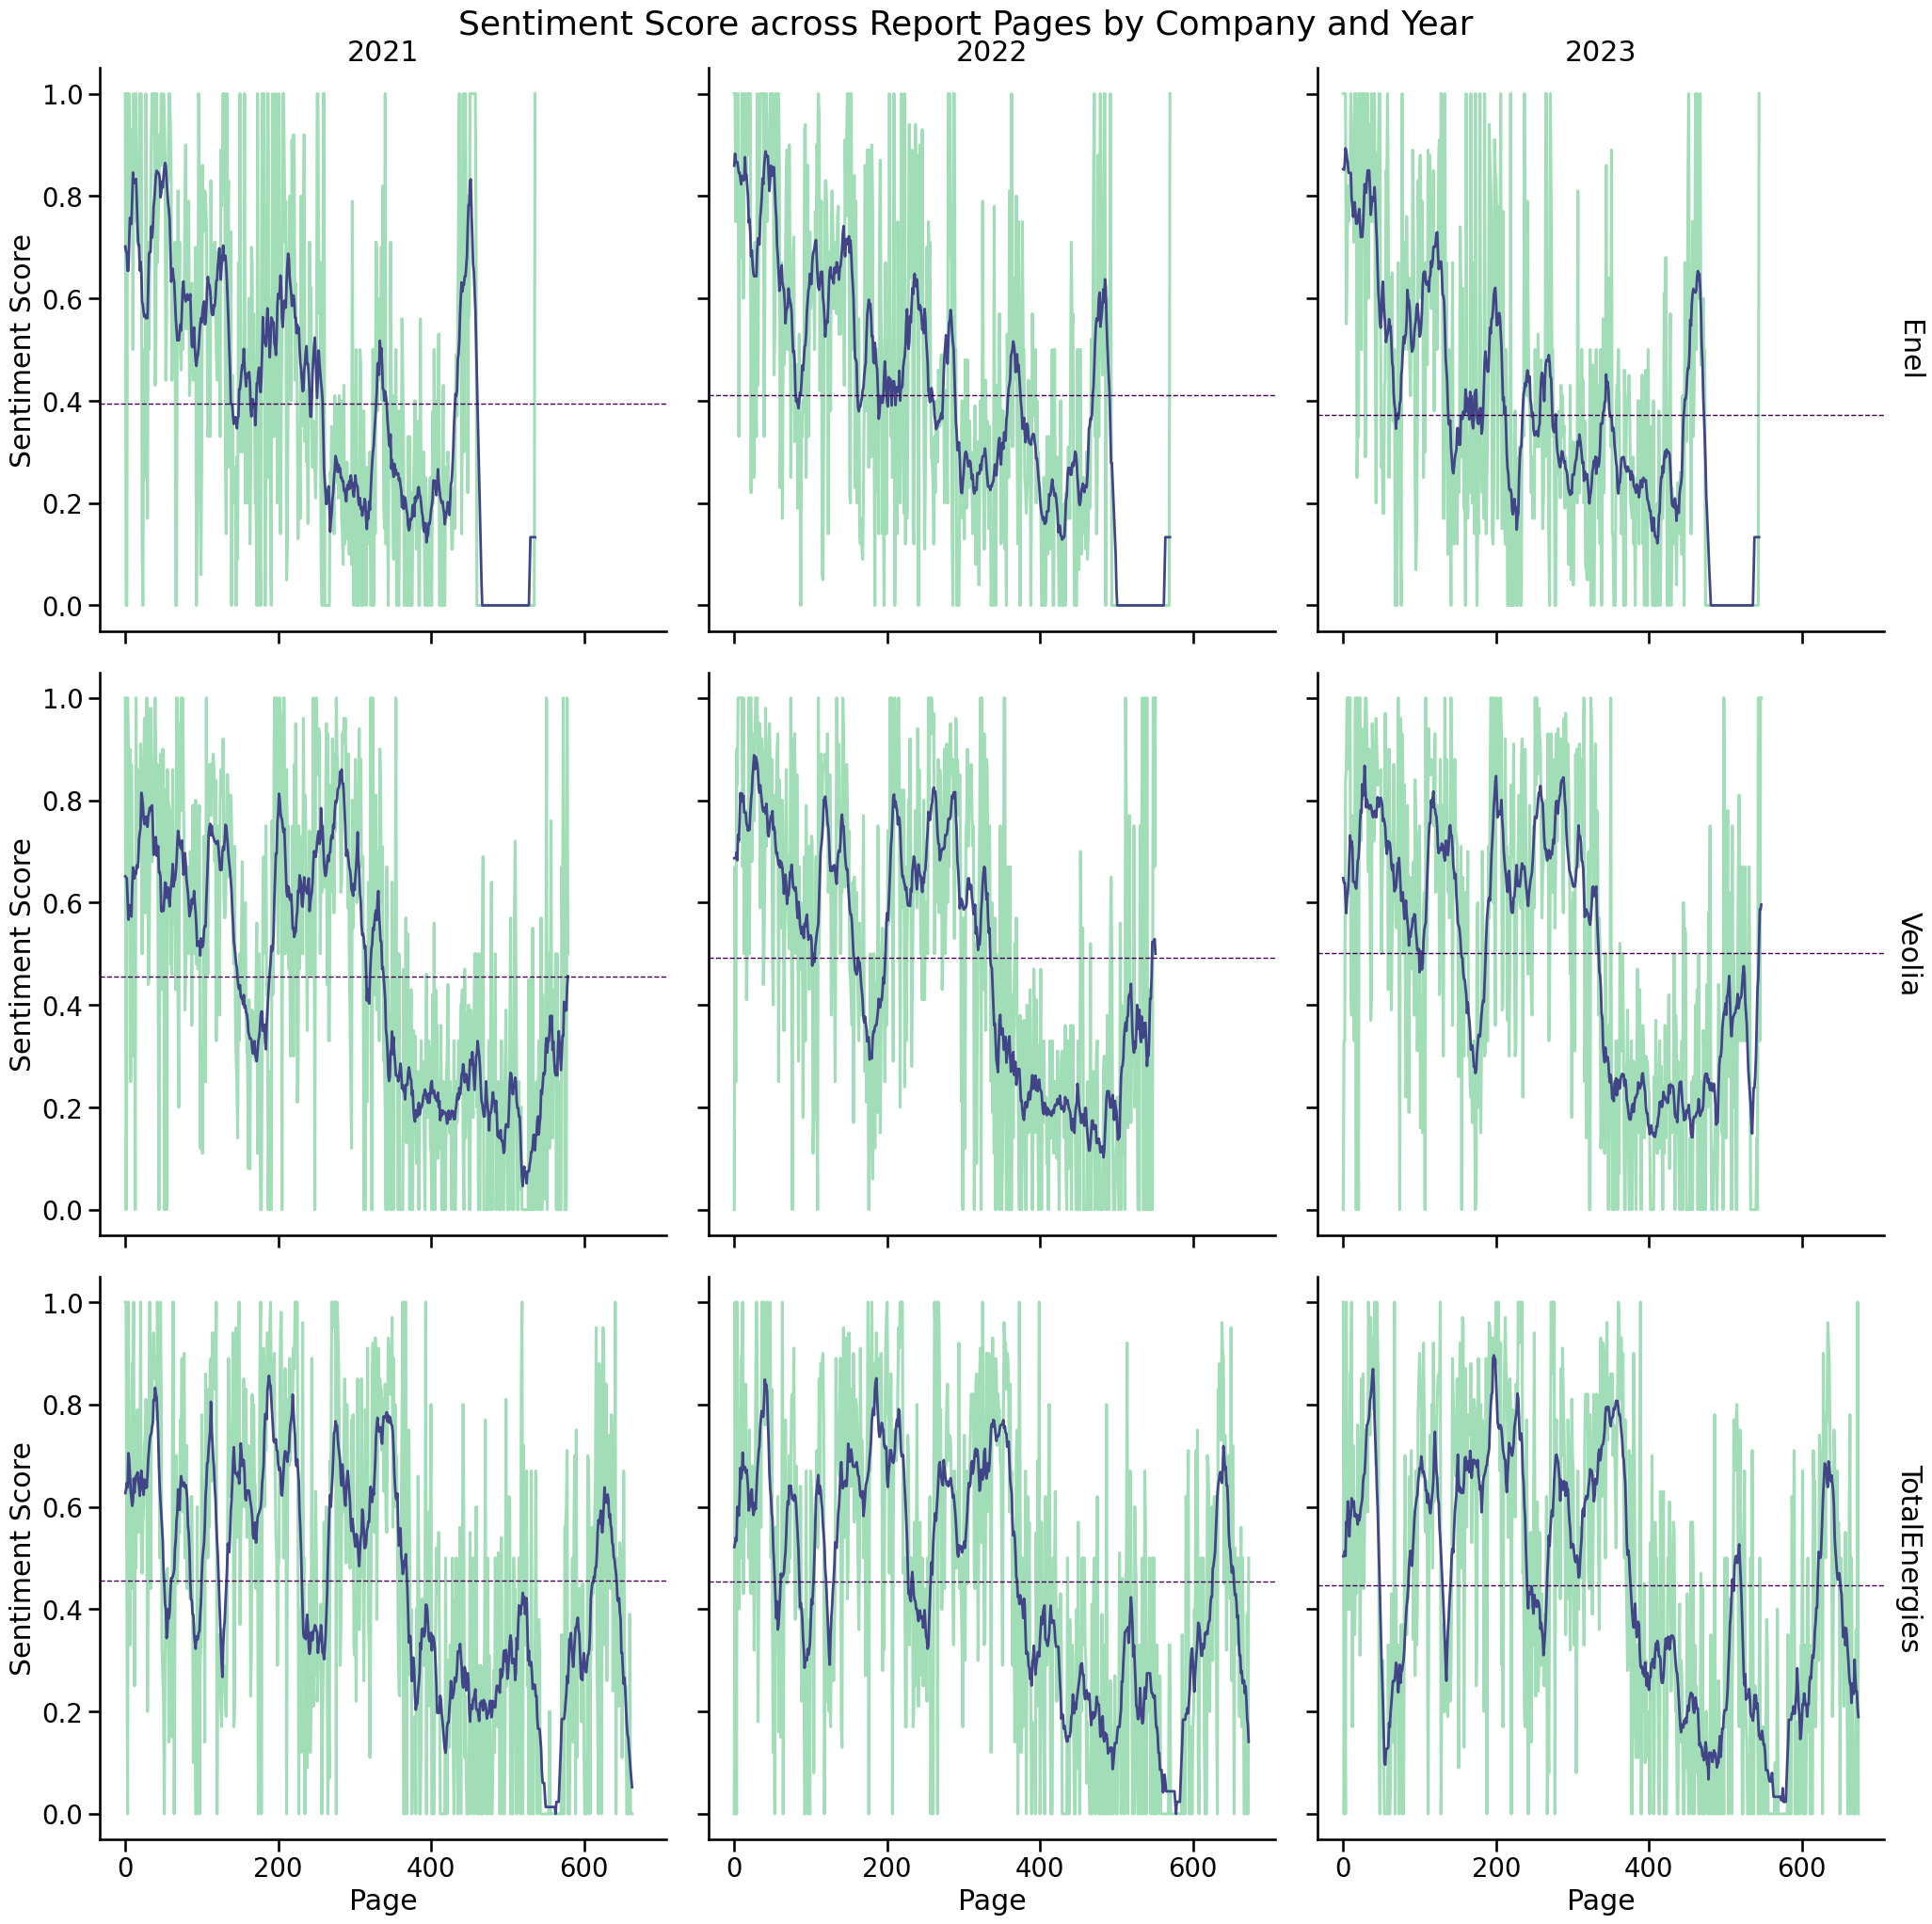
\includegraphics[width=1\linewidth]{pages1.png}
    \caption{Sentiment score per page for a sample of companies in the study. Data for three different years are shown: 2021, 2022 and 2023. The alignment values for these companies are, for Enel 33.9\% (2021), 21.4\% (2022) and 87.0\% (2023), for Veolia 0.0\% (2021), 33.1\% (2022) and 40.2\% (2023) and for TotalEnergies 1.5\% (2021), 1.3\% (2022) and 1.4\% (2023).}
    \label{fig:enter-label}
\end{figure}

\subsubsection{Sentiment Analysis and sustainability performance: weak or no significant correlation detected}
After identifying the strong dependence of the sentiment pattern on the style of each company, we proceeded to analyze in depth the relationship between the sentiment score and sustainability performance.
\par
\justify

The results, both visually and statistically, showed a weak or null correlation between sustainability performance and the sentiment score (Fig.2). The Pearson correlation analysis indicated a weak positive correlation (r=0.371, p=0.024). The Spearman correlation analysis also showed a weak positive correlation ($\rho = 0.316$) that was not statistically significant (p=0.057). Finally, the regression analysis revealed that the model explains 13.8\% of the variability in the sentiment score. That is, part of the variation in sentiment could be explained by the sustainability of the company. The F test indicates that the model is significant (p=0.024).
\par
\justify

These results are consistent with the sentiment pattern analysis and might indicate that there is no correlation between the sustainability performance of the company and the sentiment of the text. In addition, other variables could be affecting the sentiment scores. The reports used are mostly annual reports that contain not only sustainability information, but also other financial and corporate data. Therefore, these other data could mask or attenuate the sentiment due to sustainability. From a practical and application point of view, this correlation model would not allow it to be used in sentiment analysis as a proxy to understand or predict sustainability.

\begin{figure}
    \centering
    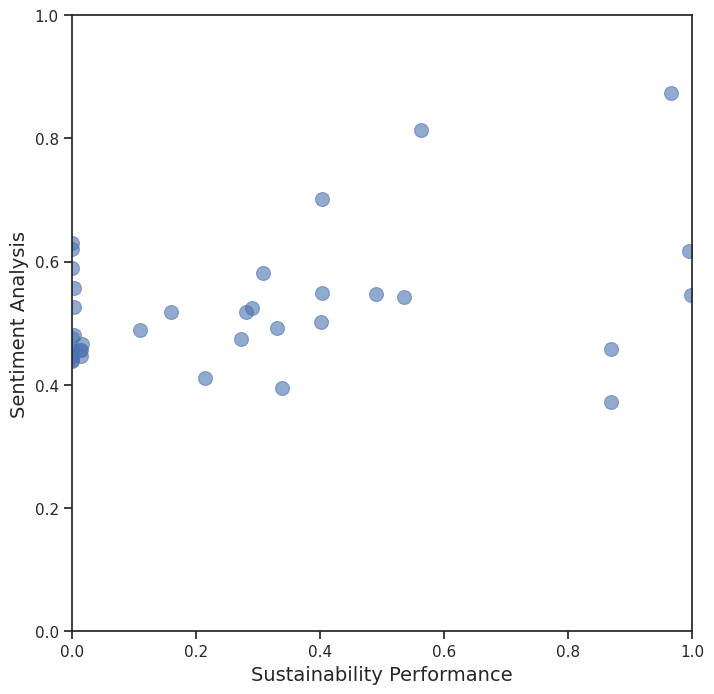
\includegraphics[width=0.5\linewidth]{corr_revenue.png}
    \caption{Sentiment analysis of the corporate report in relation to the company's sustainability performance for the specific fiscal year. The sustainability performance is measured by the company's alignment with the EU taxonomy at the revenue level.}
    \label{fig:enter-label}
\end{figure}

\begin{table}[ht]
\caption{Ordinary Least Squares (OLS) Regression Analysis Results}
\centering
\begin{tabular}{lcccccc}
\hline
\textbf{} & \textbf{coef} & \textbf{std err} & \textbf{t} & \textbf{$P>|t|$} & \textbf{[0.025} & \textbf{0.975]} \\
\hline
\textbf{const} & 0.4899 & 0.021 & 23.075 & 0.000 & 0.447 & 0.533 \\
\textbf{revenue\_alignment} & 0.1207 & 0.051 & 2.364 & 0.024 & 0.017 & 0.224 \\
\hline
\end{tabular}
\label{tab:revenue_alignment_results}
\end{table}

\subsection{Sentiment in sustainability sections: leveraging topic classification models}
After failing to identify a clear relationship between the full report sentiment and sustainability metrics, we explored the use of zero-shot topic classification models to detect the sections in which the company addresses sustainability issues. In line with sentiment, the sustainability topic score showed similar patterns over the years, also suggesting the standard structure of the text used by companies (Fig. 3)
\par
\justify
\clearpage
\begin{figure} [h]
    \centering
    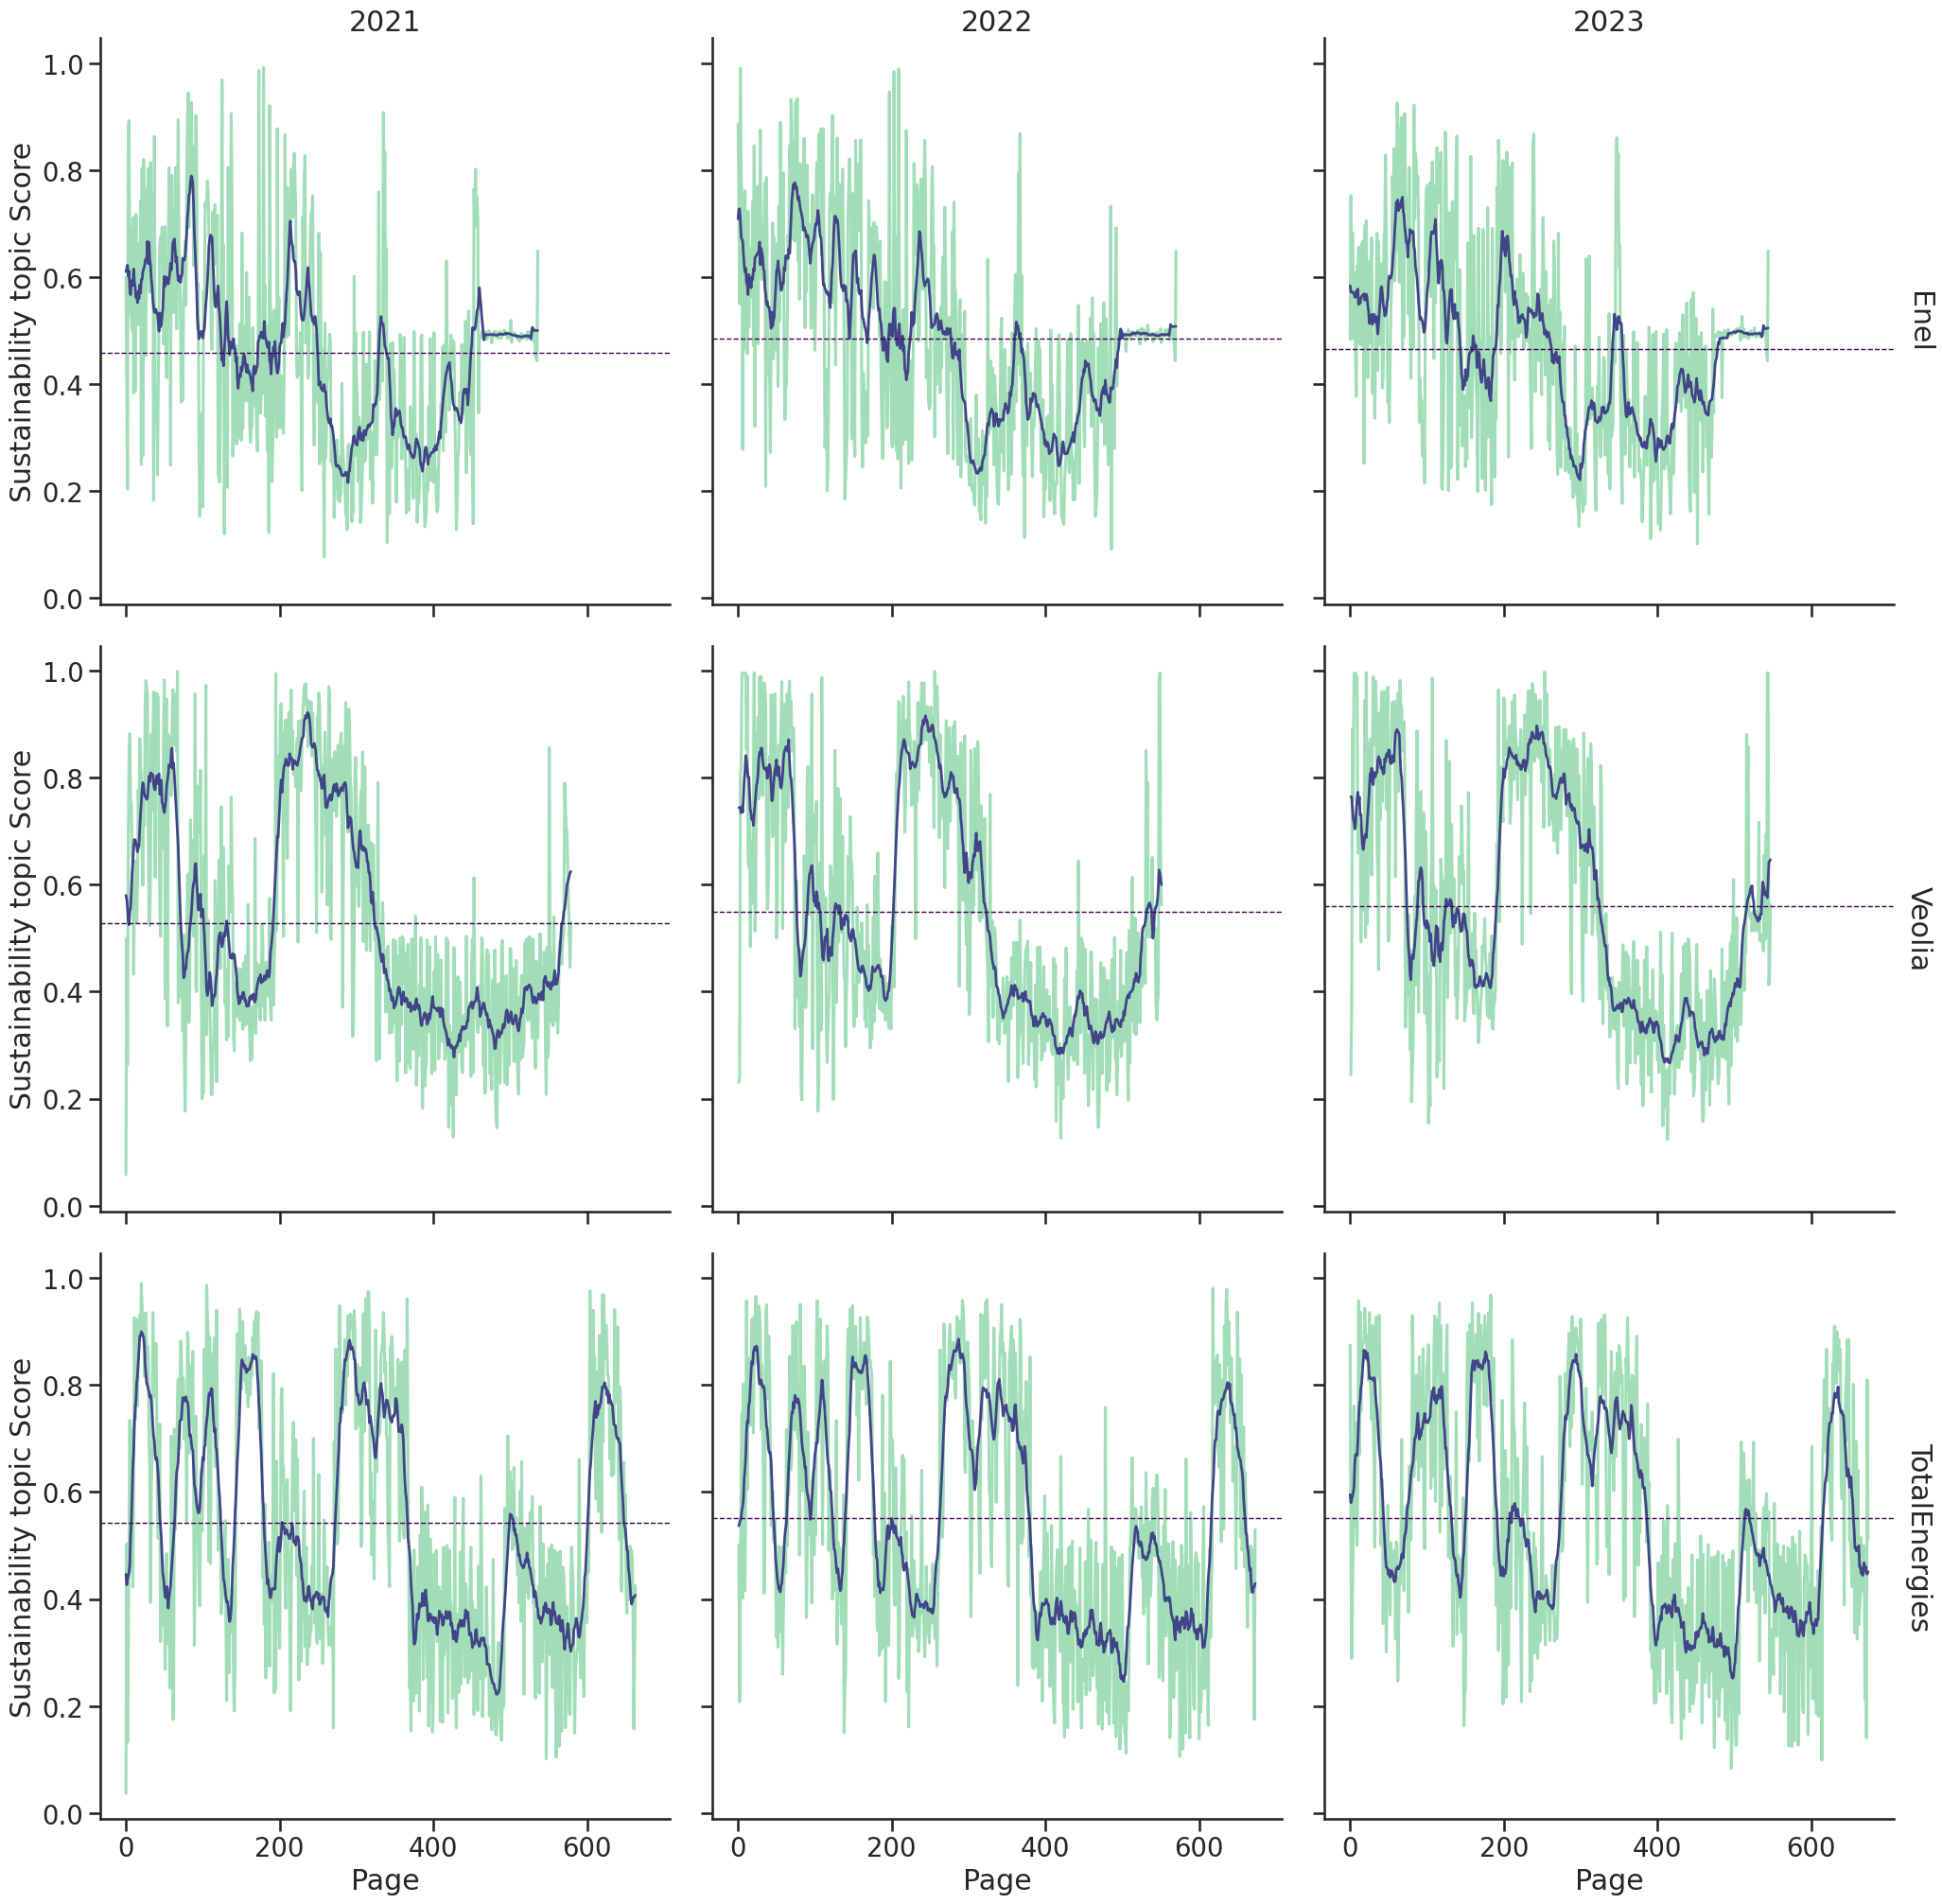
\includegraphics[width=1\linewidth]{pages2.png}
    \caption{Sustainability topic score per page for a sample of companies in the study. Data for three different years are shown: 2021, 2022 and 2023.}
    \label{fig:enter-label}
\end{figure}


We selected the 10\% of pages with the highest sustainability topic score, and analyzed the average sentiment on them. In this way we could tease out the effect of non-sustainability content, being able to explore the relationship between sentiment and sustainability by considering only the sections most related to the topic.
\par
\justify

The results indicated higher sentiment scores compared to those obtained from the full report, suggesting that the sustainability section tends to be written using more positive language. However, we observed a null or weak relationship with the sustainability metrics (Fig. 4). The Pearson correlation showed a non-significant correlation (r= 0.15, p= 0.37). According to the regression model, only 2.3\% (R-squared = 0.023) of the sentiment analysis is explained by sustainability performance if we only consider the top sustainability sections, but not significant (p-value = 0.368). These results indicate that isolating sustainability sections do not help to model sustainability performance based on sentiment analysis.

\begin{figure}
    \centering
    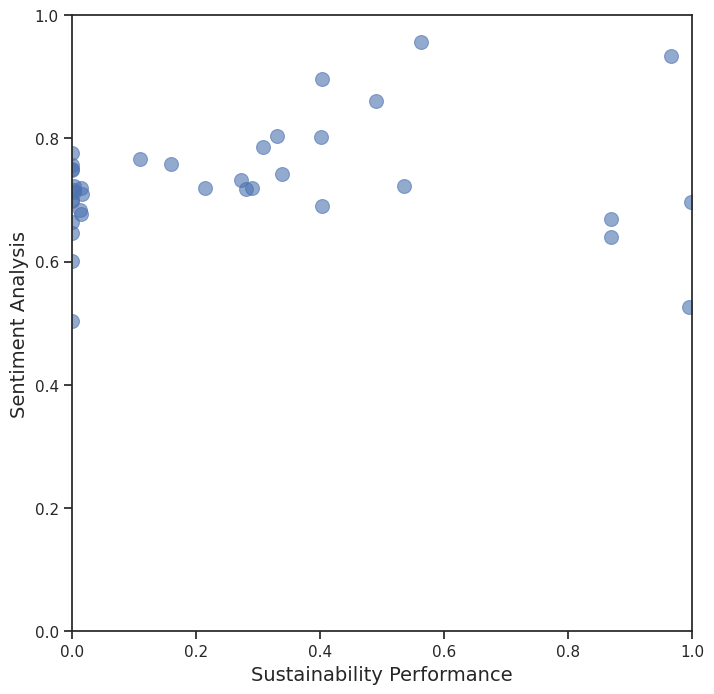
\includegraphics[width=0.5\linewidth]{corr_revenue_sust.png}
    \caption{Sentiment analysis of the sustainability sections in relation to the company’s sustainability performance for the specific fiscal year. The sustainability performance is measured by the company’s alignment with the EU taxonomy at the revenue level. Top 10\% pages with sustainability content were used for the sentiment analysis.}
    \label{fig:enter-label}
\end{figure}





%A pesar de set muy bonita la idea, los resultados de nuestra muestra demostraron que no es posible modelar la sustainability performance de la empresa utilizando el análisis de sentimiento

%limitaciones: este estudio ha sido realizado como una prueba de concepto y una muestra mayor podría arrojar más luz sobre esta relación. Sin embargo, el uso práctico de este tipo de modelos requiere una relación clara y explicable que debería haber sido advertida con la muestra utilizada. Por lo tanto, a pesar de las limitaciones del estudio, nuestros resultados sugieren que la información cualitativa contenida en los reportes no puede ser mineada utilizando análisis de sentimiento.

%Estos resultados evidencian la importancia de utilizar los datos cuantitativos de los reportes sobre los cualitativos. Therefore, modelos de extracción de información cuantitativa o iniciativas de normalización en disclosures, pueden atajar este gap de información y transparencia de una forma más eficaz.

\section{Conclusions}

Despite the potential of the proposal, the results of our sample showed that it is not possible to model the sustainability performance of the company using sentiment analysis.
\par
\justify

This study has been carried out as a proof of concept and a larger sample could shed more light on this relationship. However, the practical use of this type of model requires a clear and explainable relationship that should have been noted with the sample used. Therefore, despite the limitations of the study, our results suggest that the qualitative information contained in the reports cannot be mined using sentiment analysis.
\par
\justify

These results show the importance of using quantitative data from reports over qualitative data. Therefore, quantitative information extraction models or standardization initiatives in disclosures can address this information and transparency gap in a more effective way.
\par
\justify


\begin{thebibliography}{9}

\bibitem{european_commission_2020}
European Commission. (2020). A European Green Deal. Available at: \url{https://ec.europa.eu/info/strategy/priorities-2019-2024/european-green-deal_en}.


\bibitem{eccles_serafeim_2013}
Eccles, R. G., \& Serafeim, G. (2013). The Performance Frontier: Innovating for a Sustainable Strategy. Harvard Business Review. Available at: \url{https://hbr.org/2013/05/the-performance-frontier-innovating-for-a-sustainable-strategy}.

\bibitem{european_commission_2021}
European Commission. (2021). EU Taxonomy Regulation. Available at: \url{https://ec.europa.eu/info/business-economy-euro/banking-and-finance/sustainable-finance/eu-taxonomy-sustainable-activities_en}.

\bibitem{li2010textual}
  Li, F. (2010). The Information Content of Forward-Looking Statements in Corporate Filings—A Naïve Bayesian Machine Learning Approach. \textit{Journal of Accounting Research}, 48(5), 1049-1102. \url{https://doi.org/10.1111/j.1475-679X.2010.00382.x}.

\bibitem{kogan2009predicting}
  Kogan, S., Levin, D., Routledge, B. R., Sagi, J. S., \& Smith, N. A. (2009). Predicting risk from financial reports with regression. In \textit{Proceedings of Human Language Technologies: The 2009 Annual Conference of the North American Chapter of the Association for Computational Linguistics} (pp. 272-280). \url{https://www.aclweb.org/anthology/N09-1031/}.

\bibitem{Zao2023}
Zao, Y., Kroher, L., Engler, M. and Schnattinger, K. (2023). Detecting Greenwashing in the Environmental, Social, and Governance Domains Using Natural Language Processing. Available at: \url{https://www.scitepress.org/publishedPapers/2023/121554/pdf/index.html}.

\bibitem{Mucko2021}
Mućko, P. (2021). Sentiment analysis of CSR disclosures in annual reports of EU companies. Procedia Computer Science, 192, 3351-3359.
\url{https://www.sciencedirect.com/science/article/pii/S1877050921018470}



\bibitem{stocks}
Lindberg, M. (2022). Financial sentiment analysis of quarterly reports and stock performance. Available at: \url{https://nmbu.brage.unit.no/nmbu-xmlui/handle/11250/3021389}

\bibitem{gokturk2022}
Göktürk, G. (2022). Do Fraudulent Companies Employ Different Linguistic Features in Their Annual Reports?. Norwegian School of Economics. Available at: \url{https://openaccess.nhh.no/nhh-xmlui/bitstream/handle/11250/3015276/masterthesis.pdf?sequence=1}.










\end{thebibliography}


\appendix
\clearpage
\section*{Supplementary Figures}

\setcounter{figure}{0} % Restablecer el contador de figuras si lo deseas
\renewcommand{\thefigure}{S\arabic{figure}}

\begin{figure} [h]
    \centering
    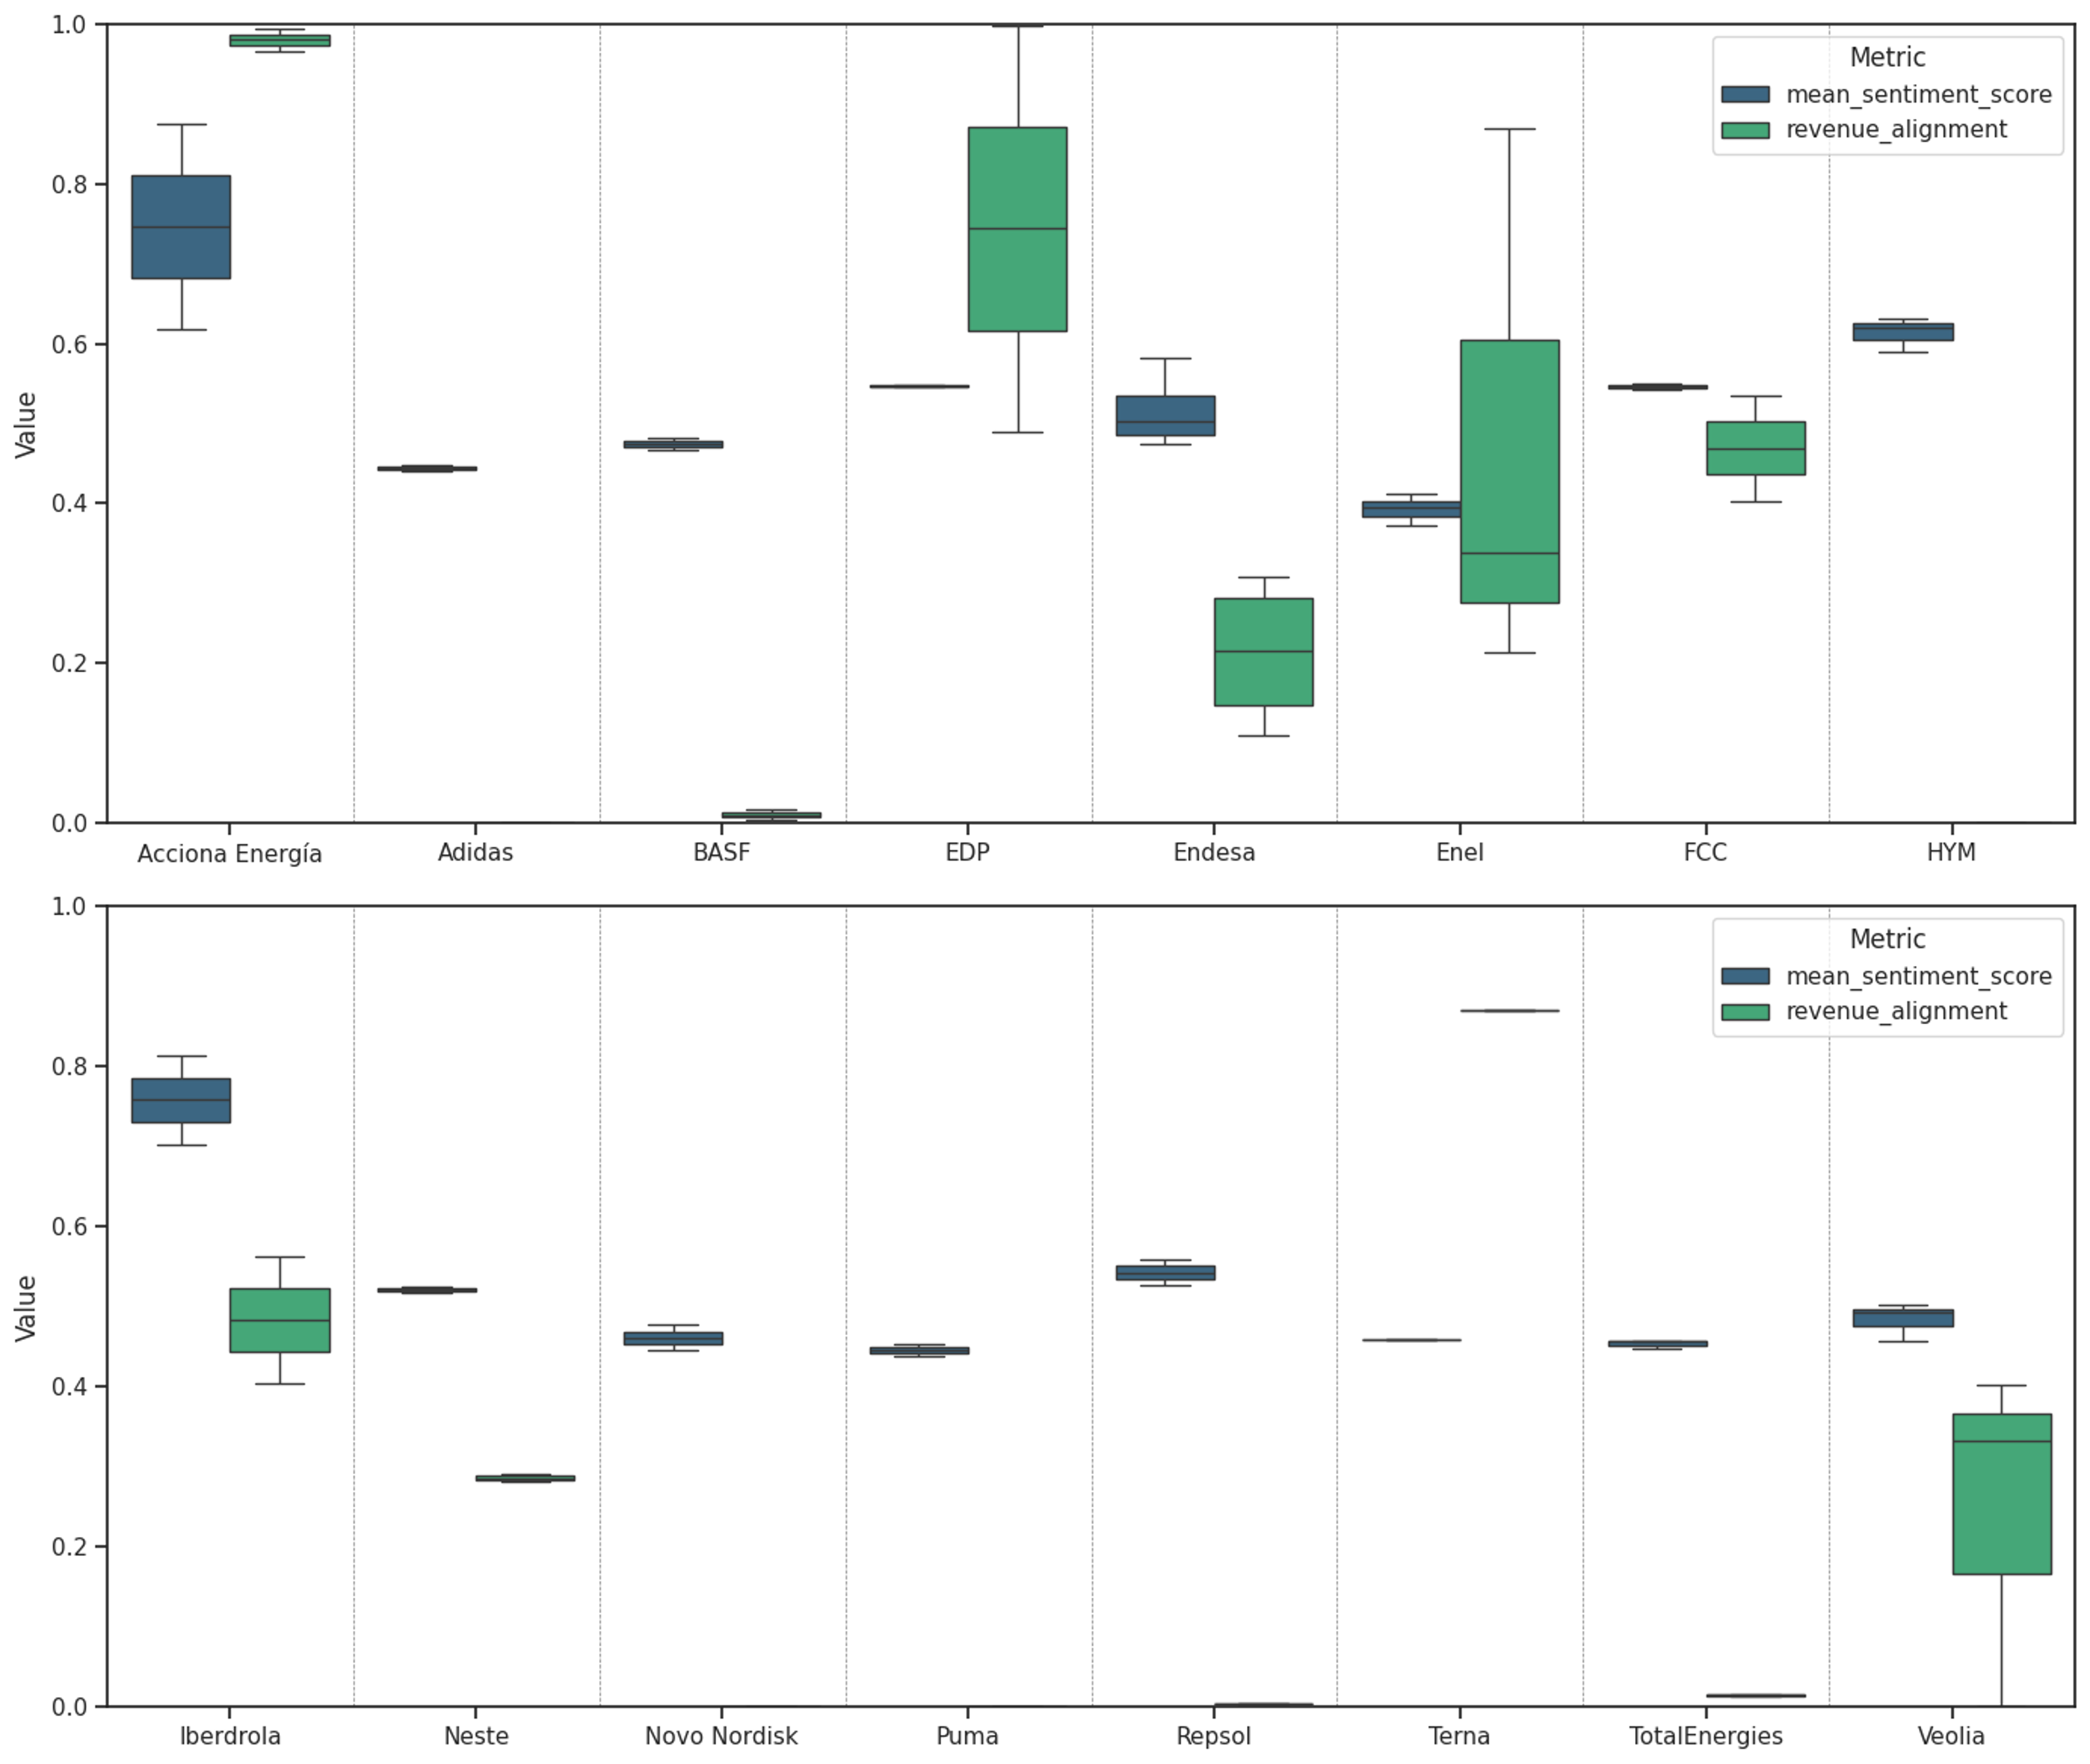
\includegraphics[width=1\linewidth]{boxplot1.png}
    \caption{Sentiment analysis and sustainability score distribution in the companies}
    \label{fig:enter-label}
\end{figure}



\begin{table}
    \centering
    \begin{tabular}{cccc}
\textbf{Company Name}      & \textbf{2021} & \textbf{2022} & \textbf{2023} \\ \hline
Iberdrola         & -     & 56.3\%      & 40.4\%     \\ \hline
EDP               & -     &   49.0\%   &  99.8\%    \\ \hline
Acciona Energía   &    99.5\%  &  96.58\%    &   -   \\ \hline
Terna             &    -  &   87.0\%   &   -   \\ \hline
Enel              &   33.9\%   &   21.4\%   &  87.0\%    \\ \hline
Veolia            &    0.0\%  &  33.1\%    &  40.2\%    \\ \hline
FCC               &    53.5\%  &  40.3\%    &   -   \\ \hline
Endesa            &    27.2\%  &  10.9\%    &  15.9\%    \\ \hline
HYM               &    0.0\%  &   0.0\%   &  0.0\%    \\ \hline
TotalEnergies     &   1.5\%   &  1.3\%    &  1.4\%    \\ \hline
Repsol            &   -   &  0.4\%    &   0.3\%   \\ \hline
BASF              &   -   &  0.4\%    &  1.6\%    \\ \hline
Adidas            &  -  &   0.0\%   &   0.0\%   \\ \hline
Puma              &   -  &   0.0\%   &   0.0\% \\ \hline
Novo Nordisk      &    -  &   0.0\%   &   0.0\% \\ \hline
Neste             &    -  &   29.0\%   &    28.0\%  \\ \hline
\end{tabular}
\caption{EU-Taxonomy alignment for the years 2021, 2022, and 2023.}
    \label{tab:my_label}
\end{table}

\end{document}